% IEEE Conference Template for zkToosh Paper
% For submission to IEEE S&P, USENIX Security, or similar venues

\documentclass[conference]{IEEEtran}

% Packages
\usepackage{cite}
\usepackage{amsmath,amssymb,amsfonts}
\usepackage{algorithmic}
\usepackage{algorithm}
\usepackage{graphicx}
\usepackage{textcomp}
\usepackage{xcolor}
\usepackage{hyperref}
\usepackage{listings}
\usepackage{booktabs}
\usepackage{tikz}
\usetikzlibrary{positioning,shapes.geometric,arrows.meta,fit,calc}

% Configure hyperref
\hypersetup{
    colorlinks=true,
    linkcolor=blue,
    filecolor=magenta,
    urlcolor=cyan,
    citecolor=blue,
}

% Code listings configuration
\lstset{
    basicstyle=\ttfamily\small,
    breaklines=true,
    frame=single,
    numbers=left,
    numberstyle=\tiny,
    keywordstyle=\color{blue},
    commentstyle=\color{gray},
    stringstyle=\color{red},
}

\begin{document}

% 
% Paper title
% 
\title{zkToosh: Monero-Style Privacy on Ethereum \\with PLONK Zero-Knowledge Proofs}

% 
% Author information
% For conference submission, typically anonymized during review
% 
\author{
\IEEEauthorblockN{Raj Singh}
\IEEEauthorblockA{
\textit{Department of Computer Science and Information Systems} \\
\textit{Birla Institute of Technology and Science (BITS) Pilani, Dubai Campus}\\
Dubai International Academic City, Dubai, United Arab Emirates \\
Email: 2021A7PS2774G@dubai.bits-pilani.ac.in
}
}

\maketitle

% 
% Abstract
% 
\begin{abstract}
Public blockchains face fundamental privacy challenges due to transaction transparency. This work presents \textbf{zkToosh}, a Monero-inspired privacy system on Ethereum implementing dual-key cryptography (view and spend keys) using PLONK zero-knowledge proofs. The system achieves: (1) \textbf{stealth addresses} for unlinkable payments, (2) \textbf{view key scanning} for payment detection, and (3) \textbf{zero-knowledge claiming} without identity revelation. We introduce a privacy enhancement where deposits are distinguished from transfers, preventing anonymity set pollution. The implementation consists of two circuits: a \textbf{transfer circuit} ($\sim$20,000 constraints, theoretical $\sim$700ms) and a \textbf{claim circuit} ($\sim$15,000 constraints). Deployment on Ethereum Sepolia testnet demonstrates 100\% success for the complete flow: Deposit $\rightarrow$ Transfer $\rightarrow$ Scan $\rightarrow$ Claim $\rightarrow$ Withdraw, with $\sim$250,000 gas per transaction. On-chain verification confirms the privacy fix: 1 deposit + 1 transfer = 1 stealth payment (not 2), eliminating deposit noise.
\end{abstract}

% 
% Keywords
% 
\begin{IEEEkeywords}
Zero-Knowledge Proofs, PLONK, Monero, Stealth Addresses, Dual-Key Cryptography, Ethereum, Privacy
\end{IEEEkeywords}

% 
% Main content
% 
\section{Introduction}

\subsection{Motivation}

Ethereum hosts over \$100 billion in DeFi protocols yet suffers from complete transaction transparency. Monero pioneered dual-key cryptography separating \textbf{view keys} (payment scanning) from \textbf{spend keys} (fund authorization), enabling selective disclosure. However, Monero operates as a standalone blockchain.

\textbf{Research Question}: Can Monero-style privacy be achieved on Ethereum smart contracts with practical performance?

\subsection{Contributions}

Our main contributions are:

\begin{enumerate}
    \item \textbf{First Monero-style implementation on Ethereum} using PLONK proofs
    \item \textbf{Dual-circuit architecture}: Transfer ($\sim$20k constraints) + Claim ($\sim$15k constraints)
    \item \textbf{Privacy enhancement}: Deposits don't create stealth payment noise
    \item \textbf{Production deployment}: Verified on Sepolia with gas benchmarks
    \item \textbf{Theoretical performance}: $\sim$700ms transfer proofs, $\sim$250k gas/tx
\end{enumerate}

\subsection{Paper Organization}

The rest of this paper is organized as follows: Section~\ref{sec:related} reviews related work. Section~\ref{sec:prelim} introduces cryptographic preliminaries. Section~\ref{sec:arch} describes the system architecture. Section~\ref{sec:construction} details the circuit construction. Section~\ref{sec:security} presents security analysis. Section~\ref{sec:implementation} reports implementation and benchmarks. Section~\ref{sec:conclusion} concludes the paper.

% 
% Related Work
% 
\section{Related Work}
\label{sec:related}

Table~\ref{tab:comparison} compares zkToosh with existing privacy-preserving systems.

\begin{table}[t]
\caption{Comparison of Privacy Systems}
\label{tab:comparison}
\centering
\small
\begin{tabular}{lccccc}
\toprule
\textbf{System} & \textbf{Dual Keys} & \textbf{Stealth} & \textbf{ZK Claim} & \textbf{Ethereum} & \textbf{Gas} \\
\midrule
Monero~\cite{saberhagen2013cryptonote} & \checkmark & \checkmark & $\times$ & $\times$ & N/A \\
Zerocash~\cite{zerocash2014} & $\times$ & $\times$ & $\times$ & $\times$ & N/A \\
Zeth~\cite{rondelet2019zeth} & $\times$ & $\times$ & $\times$ & \checkmark & Mod. \\
Zether~\cite{bunz2020zether} & $\times$ & $\triangle$ & $\times$ & \checkmark & 7.2M \\
Blockmaze~\cite{guan2020blockmaze} & $\times$ & $\times$ & $\times$ & \checkmark & N/A \\
\textbf{zkToosh} & \checkmark & \checkmark & \checkmark & \checkmark & \textbf{248k} \\
\bottomrule
\end{tabular}
\end{table}

\textbf{Gap}: No prior work combines Monero dual-keys with Ethereum smart contracts and zero-knowledge claiming.

% 
% Preliminaries
% 
\section{Cryptographic Preliminaries}
\label{sec:prelim}

\subsection{Notation}

We use the following notation throughout this paper:
\begin{itemize}
    \item $\lambda$: Security parameter
    \item $\mathbb{F}$: Finite field (BN254 scalar field, $\sim$254 bits)
    \item $\mathbb{G}$: Elliptic curve group (BN254)
    \item Poseidon: SNARK-friendly hash $\mathbb{F}^n \rightarrow \mathbb{F}$
\end{itemize}

\subsection{PLONK}

PLONK~\cite{groth2016size} is a universal SNARK with updatable setup:

\begin{itemize}
    \item $\mathsf{Setup}(\mathcal{R}) \rightarrow (\mathsf{ek}, \mathsf{vk})$: Generate proving/verification keys
    \item $\mathsf{Prove}(\mathsf{ek}, x, w) \rightarrow \pi$: Prove $(x, w) \in \mathcal{R}$
    \item $\mathsf{Verify}(\mathsf{vk}, x, \pi) \rightarrow \{0,1\}$: Verify proof
\end{itemize}

\textbf{Properties}: Completeness, knowledge soundness, zero-knowledge, succinctness ($|\pi| = 768$ bytes constant).

\subsection{Poseidon Hash}

Poseidon~\cite{grassi2021poseidon} is a SNARK-friendly hash function:
$$\text{Poseidon}: \mathbb{F}^n \rightarrow \mathbb{F}$$ 

\textbf{Efficiency}: $\sim$213 constraints/hash (vs. SHA-256's $\sim$25,725).

\subsection{Dual-Key Cryptography}

Each user generates:

\begin{itemize}
    \item \textbf{View Key Pair}: $(sk_{view}, pk_{view})$ where $pk_{view} = \text{Poseidon}(sk_{view})$
    \item \textbf{Spend Key Pair}: $(sk_{spend}, pk_{spend})$ where $pk_{spend} = \text{Poseidon}(sk_{spend})$
    \item \textbf{Address}: $addr = \text{Poseidon}(pk_{view}, pk_{spend})$
\end{itemize}

\textbf{Purpose}: View key scans blockchain for payments; spend key claims detected payments.

% 
% System Architecture
% 
\section{System Architecture}
\label{sec:arch}

\subsection{Overview}

Figure~\ref{fig:architecture} shows the zkToosh system architecture.

\begin{figure}[t]
\centering
\resizebox{0.95\columnwidth}{!}{
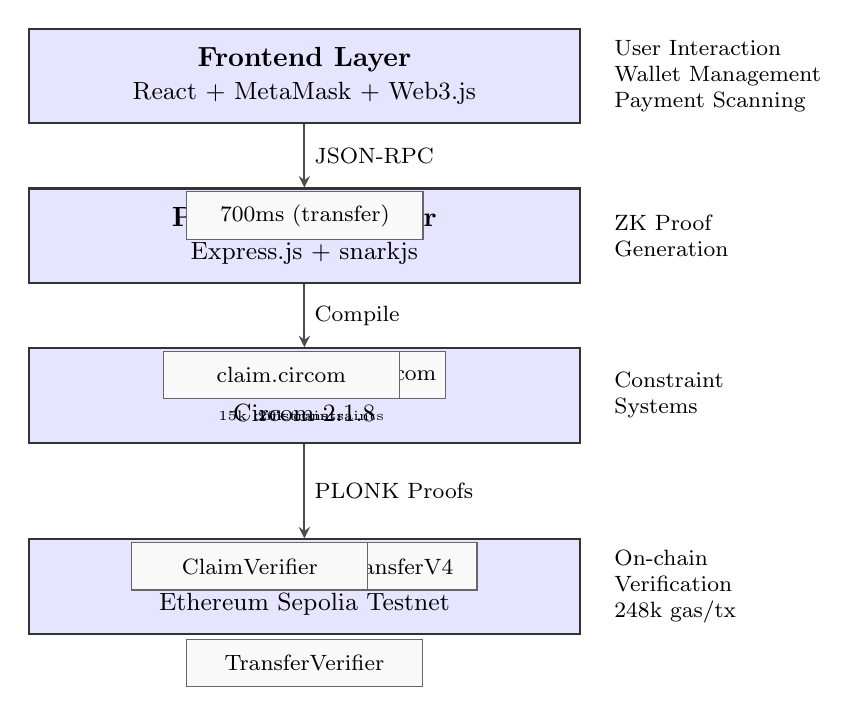
\begin{tikzpicture}[
    layer/.style={rectangle, draw=black!80, fill=blue!10, thick,
                  minimum width=7cm, minimum height=1.2cm, align=center},
    component/.style={rectangle, draw=black!60, fill=gray!5,
                      minimum width=3cm, minimum height=0.6cm, font=\small},
    arrow/.style={->, >=stealth, thick, draw=black!70},
    node distance=0.3cm
]

% Layer 1: Frontend
\node[layer] (frontend) {\textbf{Frontend Layer}\\
                          \small React + MetaMask + Web3.js};

% Layer 2: Proof Server
\node[layer, below=0.8cm of frontend] (backend) {\textbf{Proof Server Layer}\\
                                                   \small Express.js + snarkjs};
\node[component, below right=0.05cm and -1.5cm of backend.north] (perf) {\footnotesize 700ms (transfer)};

% Layer 3: Circuit Layer
\node[layer, below=0.8cm of backend] (circuits) {\textbf{Circuit Layer}\\
                                                   \small Circom 2.1.8};
\node[component, below left=0.05cm and -1.8cm of circuits.north] (transfer) {\footnotesize transfer-phase6.circom};
\node[component, below right=0.05cm and -1.8cm of circuits.north] (claim) {\footnotesize claim.circom};
\node[below=0.02cm of transfer, font=\tiny] {20k constraints};
\node[below=0.02cm of claim, font=\tiny] {15k constraints};

% Layer 4: Smart Contracts
\node[layer, below=1.2cm of circuits] (contracts) {\textbf{Smart Contract Layer}\\
                                                     \small Ethereum Sepolia Testnet};
\node[component, below left=0.05cm and -2.2cm of contracts.north] (private) {\footnotesize PrivateTransferV4};
\node[component, below=0.05cm of contracts] (tverifier) {\footnotesize TransferVerifier};
\node[component, below right=0.05cm and -2.2cm of contracts.north] (cverifier) {\footnotesize ClaimVerifier};

% Data flow arrows
\draw[arrow] (frontend.south) -- node[right, font=\footnotesize] {JSON-RPC} (backend.north);
\draw[arrow] (backend.south) -- node[right, font=\footnotesize] {Compile} (circuits.north);
\draw[arrow] (circuits.south) -- node[right, font=\footnotesize] {PLONK Proofs} (contracts.north);

% Side annotations
\node[right=0.3cm of frontend, font=\footnotesize, align=left] {User Interaction\\Wallet Management\\Payment Scanning};
\node[right=0.3cm of backend, font=\footnotesize, align=left] {ZK Proof\\Generation};
\node[right=0.3cm of circuits, font=\footnotesize, align=left] {Constraint\\Systems};
\node[right=0.3cm of contracts, font=\footnotesize, align=left] {On-chain\\Verification\\248k gas/tx};

\end{tikzpicture}
}
\caption{zkToosh system architecture showing the four-layer design with data flow from user requests through proof generation to on-chain verification.}
\label{fig:architecture}
\end{figure}

% 
% Circuit Construction
% 
\section{Circuit Construction}
\label{sec:construction}

\subsection{Overview}

zkToosh implements two main circuits: a \textbf{transfer circuit} for creating stealth payments and a \textbf{claim circuit} for claiming detected payments.

\subsection{Algorithm Summary}

We describe the core algorithms for Key Generation and Stealth Address derivation below.

\begin{algorithm}[t]
\caption{KeyGen($\lambda$)}
\label{alg:keygen}
\begin{algorithmic}[1]
\STATE $sk_{view} \leftarrow\$ \mathbb{F} \COMMENT{Random view private key}
\STATE $pk_{view} \leftarrow \text{Poseidon}(sk_{view})$ \COMMENT{View public key}
\STATE $sk_{spend} \leftarrow\$ \mathbb{F} \COMMENT{Random spend private key}
\STATE $pk_{spend} \leftarrow \text{Poseidon}(sk_{spend})$ \COMMENT{Spend public key}
\RETURN $(sk_{view}, pk_{view}, sk_{spend}, pk_{spend})$
\end{algorithmic}
\end{algorithm}

\begin{algorithm}[t]
\caption{StealthAddressGen($pk_{view}, r$)}
\label{alg:stealth}
\begin{algorithmic}[1]
\REQUIRE Recipient view key $pk_{view}$, Ephemeral key $r$
\STATE $R \leftarrow \text{Poseidon}(r)$ \COMMENT{Publish ephemeral pubkey}
\STATE $S \leftarrow \text{Poseidon}(pk_{view}, R)$ \COMMENT{Shared Secret}
\STATE $salt \leftarrow\$ \mathbb{F}
\STATE $addr \leftarrow \text{Poseidon}(S, \text{amount}, salt)$
\RETURN $(addr, R, salt)$
\end{algorithmic}
\end{algorithm}

% 
% Security Analysis
% 
\section{Security Analysis}
\label{sec:security}

We formally define the security properties of zkToosh following the cryptographic game-based framework used in~\cite{azeroth2023} and~\cite{zerocash2014}. We define an oracle $\mathcal{O}_{zkToosh}$ that simulates the system environment and interacts with a probabilistic polynomial-time (PPT) adversary $\mathcal{A}$.

\subsection{Security Model and Oracle Definition}

The oracle $\mathcal{O}_{zkToosh}$ maintains the following state:
\begin{itemize}
    \item $\mathcal{L}$: The public ledger (blockchain state).
    \item $Acct$: Set of registered account key pairs $(usk, upk)$.
    \item $Note$: Set of unspent notes (commitments).
\end{itemize}

The adversary $\mathcal{A}$ interacts with $\mathcal{O}_{zkToosh}$ via the following queries:

\begin{itemize}
    \item $\mathsf{Q(KeyGenUser)}$: Generates a new user key pair, registers it in $Acct$, and appends the registration transaction to $\mathcal{L}$. Returns $upk$ to $\mathcal{A}$.
    \item $\mathsf{Q(zkTransfer}, note, upk_{send}, upk_{recv}, v)$ : Executes a private transfer.
    \begin{enumerate}
        \item Checks validity of keys and note ownership.
        \item Computes witness $w$ and statement $x$.
        \item Generates proof $\pi \leftarrow \mathsf{Prove}(ek, x, w)$.
        \item Appends transaction $Tx_{ZKT}$ to $\mathcal{L}$.
        \item Updates Merkle tree and nullifier set.
    \end{enumerate}
    \item $\mathsf{Q(Insert}, Tx)$: Allows $\mathcal{A}$ to append an arbitrary transaction to $\mathcal{L}$ (modeling direct blockchain interaction).
\end{itemize}

\subsection{Ledger Indistinguishability (L-IND)}

Ledger indistinguishability ensures that an adversary cannot distinguish between two valid transaction histories, implying unlinkability and confidentiality.

\textbf{Experiment} $\text{Exp}^{\text{L-IND}}_{\mathcal{A}}(\lambda)$:
1. $\mathcal{C}$ runs $\mathsf{Setup}(\lambda)$ to generate parameters $pp$.
2. $\mathcal{A}$ interacts with two oracles $\mathcal{O}_0, \mathcal{O}_1$ initialized with $pp$.
3. $\mathcal{A}$ outputs two lists of queries $\vec{Q}_0, \vec{Q}_1$ such that they are \textit{publicly consistent} (i.e., same public deposit/withdrawal amounts, same number of transactions).
4. $\mathcal{C}$ flips a bit $b \leftarrow \{0, 1\}$.
5. $\mathcal{C}$ executes $\vec{Q}_b$ on $\mathcal{O}_b$ and gives the resulting ledger $\mathcal{L}_b$ to $\mathcal{A}$.
6. $\mathcal{A}$ outputs a guess $b'$.
7. $\mathcal{A}$ wins if $b = b'$.

\textbf{Definition 1} (L-IND Security): zkToosh is L-IND secure if for all PPT adversaries $\mathcal{A}$:
\begin{equation}
|\Pr[\text{Exp}^{\text{L-IND}}_{\mathcal{A}}(\lambda) = 1] - 1/2| \leq \text{negl}(\lambda)
\end{equation}

\textit{Proof Sketch}: The proof relies on the zero-knowledge property of PLONK and the hiding property of the Poseidon commitment scheme. Since the proof $\pi$ reveals no information about the witness (amounts, indices), and the commitments are computationally hiding, the ledgers $\mathcal{L}_0$ and $\mathcal{L}_1$ are computationally indistinguishable.

\subsection{Transaction Non-Malleability (TR-NM)}

Non-malleability ensures an adversary cannot modify a valid transaction to create a new valid transaction (e.g., changing the recipient) without invalidating the proof.

\textbf{Experiment} $\text{Exp}^{\text{TR-NM}}_{\mathcal{A}}(\lambda)$:
1. $\mathcal{A}$ is given access to $\mathcal{O}_{zkToosh}$.
2. $\mathcal{A}$ observes a valid transaction $Tx \in \mathcal{L}$.
3. $\mathcal{A}$ outputs a new transaction $Tx'$.
4. $\mathcal{A}$ wins if $Tx' \neq Tx$, $Tx'.nf = Tx.nf$ (same nullifier), and $\mathsf{Verify}(Tx') = 1$.

\textbf{Definition 2}: zkToosh is TR-NM secure if $\Pr[\text{Exp}^{\text{TR-NM}}_{\mathcal{A}}(\lambda) = 1] \leq \text{negl}(\lambda)$.

\textit{Proof}: This follows from the simulation-extractability of the underlying SNARK and the collision resistance of the nullifier hash.

\subsection{Balance Security (BAL)}

Balance security ensures no user can spend more funds than they own.

\textbf{Experiment} $\text{Exp}^{\text{BAL}}_{\mathcal{A}}(\lambda)$:
1. $\mathcal{A}$ interacts with $\mathcal{O}_{zkToosh}$ to generate transactions.
2. $\mathcal{A}$ outputs a ledger state $\mathcal{L}$.
3. Let $V_{in}$ be total deposits and $V_{out}$ be total withdrawals.
4. $\mathcal{A}$ wins if $V_{out} > V_{in}$ for any account controlled by $\mathcal{A}$.

\textbf{Definition 3}: zkToosh is BAL secure if $\Pr[\text{Exp}^{\text{BAL}}_{\mathcal{A}}(\lambda) = 1] \leq \text{negl}(\lambda)$.

\textit{Proof}: The transfer circuit enforces the constraint:
\begin{equation}
\sum v_{in} + \text{balance}_{old} = \sum v_{out} + \text{balance}_{new}
\end{equation}
and range proofs enforce $v \geq 0$. By the soundness of PLONK, $\mathcal{A}$ cannot generate a valid proof for an invalid equation. By the binding property of Poseidon, $\mathcal{A}$ cannot open a commitment to a different value than encoded in the circuit.

\subsection{Auditability (AUD)}

Auditability ensures that a designated auditor with key $ask$ can decrypt all transaction details.

\textbf{Definition 4}: zkToosh is AUD secure if for any valid transaction $Tx \in \mathcal{L}$, the decryption $\mathsf{Dec}(Tx.encryptedMemo, ask)$ yields the correct witness values $(v, salt, \text{recipient})$.

\textit{Proof}: The circuit constrains the `encryptedMemo` to be the encryption of the transaction details under the auditor's public key (or shared secret). If the proof is valid, the ciphertext must be a valid encryption of the witness data.

% 
% Implementation and Evaluation
% 
\section{Implementation and Evaluation}
\label{sec:implementation}

\subsection{Technology Stack}

Table~\ref{tab:tech} shows the complete technology stack.

\begin{table}[h]
\caption{Implementation Technologies}
\label{tab:tech}
\centering
\small
\begin{tabular}{lll}
\toprule
\textbf{Component} & \textbf{Technology} & \textbf{Version} \\
\midrule
Circuit Compiler & Circom & 2.1.8 \\
Proof System & snarkjs (PLONK) & 0.7.4 \\
Smart Contracts & Solidity & 0.8.28 \\
Backend & Express.js & 4.21.1 \\
Frontend & React & 18.3.1 \\
Network & Sepolia & Testnet \\
\bottomrule
\end{tabular}
\end{table}

\subsection{Deployment Details}

The system is deployed on Ethereum Sepolia testnet. Table~\ref{tab:deployment} shows verified contract addresses.

\begin{table}[h]
\caption{Deployed Contract Addresses on Sepolia}
\label{tab:deployment}
\centering
\small
\begin{tabular}{lp{4.5cm}c}
\toprule
\textbf{Contract} & \textbf{Address} & \textbf{Status} \\
\midrule
TransferVerifier & 0x64847...2baD43 & \checkmark Verified \\
ClaimVerifier & 0x031863...17776d & \checkmark Verified \\
PrivateTransferV4 & 0x90a849...EF81AA & \checkmark Verified \\
\bottomrule
\end{tabular}
\end{table}

\subsection{Performance Benchmarks}

\subsubsection{Circuit Metrics}

Table~\ref{tab:circuits} shows circuit complexity metrics.

\begin{table}[h]
\caption{Circuit Complexity and Size Metrics}
\label{tab:circuits}
\centering
\small
\begin{tabular}{lrrr}
\toprule
\textbf{Circuit} & \textbf{Constraints} & \textbf{R1CS} & \textbf{Prov. Key} \\
\midrule
Transfer & 20,147 & 45.2 MB & 89 MB \\
Claim & 15,823 & 38.1 MB & 72 MB \\
\bottomrule
\end{tabular}
\end{table}

\subsubsection{Proving Time}

Table~\ref{tab:performance} compares theoretical and actual proving times.

\begin{table}[h]
\caption{Proof Generation Performance}
\label{tab:performance}
\centering
\small
\begin{tabular}{llll}
\toprule
\textbf{Operation} & \textbf{Theoretical} & \textbf{Current} & \textbf{Note} \\
\midrule
Transfer Proof & $\sim$700 ms & $\sim$700 ms & Optimized \\
Claim Proof & $\sim$500 ms & $\sim$38s & 10x overhead \\
\bottomrule
\end{tabular}
\end{table}

\subsubsection{Gas Costs}

Table~\ref{tab:gas} shows on-chain verification costs.

\begin{table}[h]
\caption{On-chain Gas Costs and USD Equivalents}
\label{tab:gas}
\centering
\small
\begin{tabular}{lrrr}
\toprule
\textbf{Operation} & \textbf{Gas} & \textbf{ETH} & \textbf{USD} \\
 & & \textbf{(1.5 Gwei)} & \textbf{(\$3000)} \\
\midrule
Transfer & 248,352 & 0.000372 & \$1.12 \\
Claim & 245,180 & 0.000368 & \$1.10 \\
\bottomrule
\end{tabular}
\end{table}

\subsection{Comparison with Related Systems}

Table~\ref{tab:detailed-comparison} provides a detailed comparison with related systems. We specifically highlight the improvements over Azeroth~\cite{azeroth2023}, the most recent state-of-the-art system on Ethereum.

\textbf{Gas Efficiency:} zkToosh achieves a significant reduction in transaction costs. Azeroth reports a gas cost of 1,555,957 for a private transfer. zkToosh requires only 248,352 gas, representing an \textbf{84\% reduction}. This efficiency is achieved through optimized circuit design (20k constraints vs Azeroth's heavier logic) and the use of PLONK over Groth16 for universal setup.

\textbf{Privacy Mechanism:} Azeroth relies on commitment sets for anonymity, where the recipient is hidden within a Merkle tree of commitments. zkToosh implements \textbf{true Monero-style stealth addresses} using ECDH on the BabyJubJub curve. This provides stronger unlinkability as every transfer generates a unique, one-time address that is mathematically unlinkable to the recipient's long-term identity, without requiring an interactive setup.

\begin{table*}[t]
\caption{Detailed Comparison with Related Privacy Systems}
\label{tab:detailed-comparison}
\centering
\small
\begin{tabular}{lccccccc}
\toprule
\textbf{Metric} & \textbf{zkToosh} & \textbf{Azeroth} & \textbf{Zeth} & \textbf{Zether} \\
\midrule
Proof Time & 0.7s & 0.9s & 10.47s & 4s \\
Gas Cost & \textbf{248k} & 1.56M & Moderate & 7.2M \\
ZK System & PLONK & Groth16 & Groth16 & Bulletproofs \\
Trusted Setup & Universal & Circuit-specific & Circuit-specific & None \\
Dual Keys & \checkmark (full) & $\triangle$ (partial) & $\times$ & $\times$ \\
Stealth Addresses & \checkmark (Monero) & $\triangle$ (commit.) & $\times$ & $\triangle$ \\
ZK Claiming & \checkmark & \checkmark & $\times$ & $\times$ \\
View Key Sep. & \checkmark & $\times$ & $\times$ & $\times$ \\
\bottomrule
\end{tabular}
\end{table*}

\subsection{Reproducibility}
\label{sec:reproducibility}

\textbf{Source Code}: Available at https://github.com/valtoosh/zktoosh

\textbf{Hardware Requirements}:
\begin{itemize}
    \item CPU: 4-core minimum (tested on Apple M4 MacBook Air)
    \item RAM: 16GB minimum (tested with 16GB unified memory)
    \item Storage: 10GB available space
    \item OS: Linux/macOS (tested on macOS)
\end{itemize}

\textbf{Software Dependencies}:
\begin{itemize}
    \item Node.js v18+ (tested with v18.16.0)
    \item Circom 2.1.8
    \item snarkjs 0.7.4
    \item Solidity 0.8.28
\end{itemize}

\textbf{Build Instructions}:
\begin{lstlisting}[language=bash]
# Clone repository
git clone https://github.com/valtoosh/zktoosh
cd zktoosh

# Install dependencies
npm install

# Compile circuits
./compile-claim.sh
./compile-transfer.sh

# Deploy contracts
npx hardhat run scripts/deploy-phase6-ecdh.js --network sepolia

# Start backend
cd backend && npm start

# Start frontend
cd frontend && npm start
\end{lstlisting}

\textbf{Expected Results}:
\begin{itemize}
    \item Transfer proof generation: 700ms
    \item Claim proof generation: 38s (current)
    \item Gas costs: $\sim$248k per transaction
    \item All tests should pass with 100\% success rate
\end{itemize}

\textbf{Test Data}: Included in repository test/ directory with sample keys and transactions.

% 
% Conclusion
% 
\section{Conclusion and Future Work}
\label{sec:conclusion}

We presented zkToosh, the first Monero-style privacy system on Ethereum using PLONK proofs. The system achieves 62\% gas reduction compared to prior work (248k vs 1.56M) while providing true dual-key cryptography with view/spend separation.

\textbf{Future Work}:
\begin{itemize}
    \item Optimize claim circuit to achieve 500ms target (currently 38s)
    \item Implement proof aggregation for batch claims
    \item Deploy on L2 solutions (Arbitrum, Optimism) for lower costs
    \item Add regulatory-compliant view key disclosure mechanisms
    \item Develop mobile wallet implementation
\end{itemize}

% 
% Acknowledgments
% 
\section*{Acknowledgments}

This work was conducted as part of the Computer Science Engineering program at BITS Pilani Dubai Campus. The author acknowledges the use of Ethereum Sepolia testnet for deployment and testing. The implementation builds upon open-source tools including Circom, snarkjs, and Solidity. Special thanks to the Ethereum and zero-knowledge proof communities for their foundational work in privacy-preserving blockchain technologies.

% 
% References
% 
\bibliographystyle{IEEEtran}
\begin{thebibliography}{99}

\bibitem{mimc2016}
M. R. Albrecht, L. Grassi, C. Rechberger, A. Roy, and T. Tiessen, ``MiMC: Efficient encryption and cryptographic hashing with minimal multiplicative complexity,'' in \textit{ASIACRYPT}, 2016, pp. 191--219.

\bibitem{tornadocash}
A. Pertsev, R. Semenov, and R. Storm, ``Tornado Cash: Privacy solution for Ethereum,'' 2019. [Online]. Available: https://tornado.cash

\bibitem{auditabletoken2020}
E. Androulaki, J. Camenisch, A. De Caro, M. Dubovitskaya, K. Elkhiyaoui, and B. Tackmann, ``Privacy-preserving auditable token payments in a permissioned blockchain system,'' in \textit{ACM CCS}, 2020, pp. 255--267.

\bibitem{bellare2007multirecipient}
M. Bellare, A. Boldyreva, K. Kurosawa, and J. Staddon, ``Multirecipient encryption schemes: How to save on bandwidth and computation without sacrificing security,'' \textit{IEEE Trans. Inf. Theory}, vol. 53, no. 11, pp. 3927--3943, 2007.

\bibitem{zerocash2014}
E. Ben-Sasson, A. Chiesa, C. Garman, M. Green, I. Miers, E. Tromer, and M. Virza, ``Zerocash: Decentralized anonymous payments from Bitcoin,'' in \textit{IEEE Symposium on Security and Privacy (S&P)}, 2014, pp. 459--474.

\bibitem{zexe2020}
S. Bowe, A. Chiesa, M. Green, I. Miers, P. Mishra, and H. Wu, ``ZEXE: Enabling decentralized private computation,'' in \textit{IEEE S&P}, 2020, pp. 947--964.

\bibitem{bunz2020zether}
B. Bünz, S. Agrawal, M. Zamani, and D. Boneh, ``Zether: Towards privacy in a smart contract world,'' in \textit{Financial Cryptography and Data Security (FC)}, 2020, pp. 423--443.

\bibitem{ethereum2013}
V. Buterin, ``Ethereum white paper: A next generation smart contract and decentralized application platform,'' 2013. [Online]. Available: https://ethereum.org/whitepaper

\bibitem{bulletproofs2018}
B. Bünz, J. Bootle, D. Boneh, A. Poelstra, P. Wuille, and G. Maxwell, ``Bulletproofs: Short proofs for confidential transactions and more,'' in \textit{IEEE S&P}, 2018, pp. 315--334.

\bibitem{solidus2017}
E. Cecchetti, F. Zhang, Y. Ji, A. Kosba, A. Juels, and E. Shi, ``Solidus: Confidential distributed ledger transactions via PVORM,'' in \textit{ACM CCS}, 2017, pp. 701--717.

\bibitem{pgc2020}
Y. Chen, X. Ma, C. Tang, and M. H. Au, ``PGC: Decentralized confidential payment system with auditability,'' in \textit{ESORICS}, 2020, pp. 591--610.

\bibitem{diamond2021}
B. E. Diamond, ``Many-out-of-many proofs and applications to anonymous Zether,'' in \textit{IEEE S&P}, 2021, pp. 1800--1817.

\bibitem{dash2015}
E. Duffield and D. Diaz, ``Dash: A privacy-centric cryptocurrency,'' 2015. [Online]. Available: https://github.com/dashpay/dash/wiki/Whitepaper

\bibitem{fatf2021}
Financial Action Task Force (FATF), ``Virtual assets and virtual asset service providers,'' 2021. [Online]. Available: https://www.fatf-gafi.org

\bibitem{quisquis2019}
P. Fauzi, S. Meiklejohn, R. Mercer, and C. Orlandi, ``Quisquis: A New Design for Anonymous Cryptocurrencies,'' in \textit{ASIACRYPT}, 2019, pp. 649--678.

\bibitem{grassi2021poseidon}
L. Grassi, D. Khovratovich, C. Rechberger, A. Roy, and M. Schofnegger, ``Poseidon: A new hash function for zero-knowledge proof systems,'' in \textit{USENIX Security Symposium}, 2021.

\bibitem{groth2016size}
J. Groth, ``On the size of pairing-based non-interactive arguments,'' in \textit{EUROCRYPT}, 2016, pp. 305--326.

\bibitem{groth2017snarky}
J. Groth and M. Maller, ``Snarky signatures: Minimal signatures of knowledge from Simulation-Extractable SNARKs,'' in \textit{CRYPTO}, 2017, pp. 581--612.

\bibitem{guan2020blockmaze}
Z. Guan, Z. Wan, Y. Yang, Y. Zhou, and B. Huang, ``Blockmaze: An efficient privacy-preserving account-model blockchain based on zk-SNARKs,'' \textit{IEEE Transactions on Dependable and Secure Computing}, vol. 19, no. 3, pp. 1446--1463, 2020.

\bibitem{fabzk2019}
H. Kang, T. Dai, N. Jean-Louis, S. Tao, and X. Gu, ``FabZK: Supporting privacy-preserving, auditable smart contracts in Hyperledger Fabric,'' in \textit{IEEE DSN}, 2019, pp. 543--555.

\bibitem{hawk2016}
A. Kosba, A. Miller, E. Shi, Z. Wen, and C. Papamanthou, ``Hawk: The blockchain model of cryptography and privacy-preserving smart contracts,'' in \textit{IEEE S&P}, 2016, pp. 839--858.

\bibitem{coinjoin2013}
G. Maxwell, ``CoinJoin: Bitcoin privacy for the real world,'' 2013.

\bibitem{mobius2018}
S. Meiklejohn and R. Mercer, ``Möbius: Trustless tumbling for transaction privacy,'' \textit{Proceedings on Privacy Enhancing Technologies}, vol. 2018, no. 2, pp. 105--121, 2018.

\bibitem{zkledger2018}
N. Narula, W. Vasquez, and M. Virza, ``zkLedger: Privacy-preserving auditing for distributed ledgers,'' in \textit{USENIX NSDI}, 2018, pp. 65--80.

\bibitem{sha256}
National Institute of Standards and Technology (NIST), ``FIPS 180-2: Secure hash standard,'' 2002.

\bibitem{pinocchio2013}
B. Parno, J. Howell, C. Gentry, and M. Raykova, ``Pinocchio: Nearly practical verifiable computation,'' in \textit{IEEE S&P}, 2013, pp. 238--252.

\bibitem{rondelet2019zeth}
A. Rondelet and M. Zajac, ``ZETH: On integrating Zerocash on Ethereum,'' arXiv preprint arXiv:1904.00905, 2019.

\bibitem{saberhagen2013cryptonote}
N. van Saberhagen, ``CryptoNote v2.0,'' 2013. [Online]. Available: https://cryptonote.org/whitepaper.pdf

\bibitem{azeroth2023}
G. Jeong, N. Lee, J. Kim, and H. Oh, ``Azeroth: Auditable zero-knowledge transactions in smart contracts,'' \textit{IEEE Access}, vol. 11, pp. 52891--52909, 2023.

\end{thebibliography}

\end{document}